\documentclass[11pt]{report}
\usepackage{tikz}
\usetikzlibrary{fit,positioning}
\begin{document}

\begin{figure}
\centering
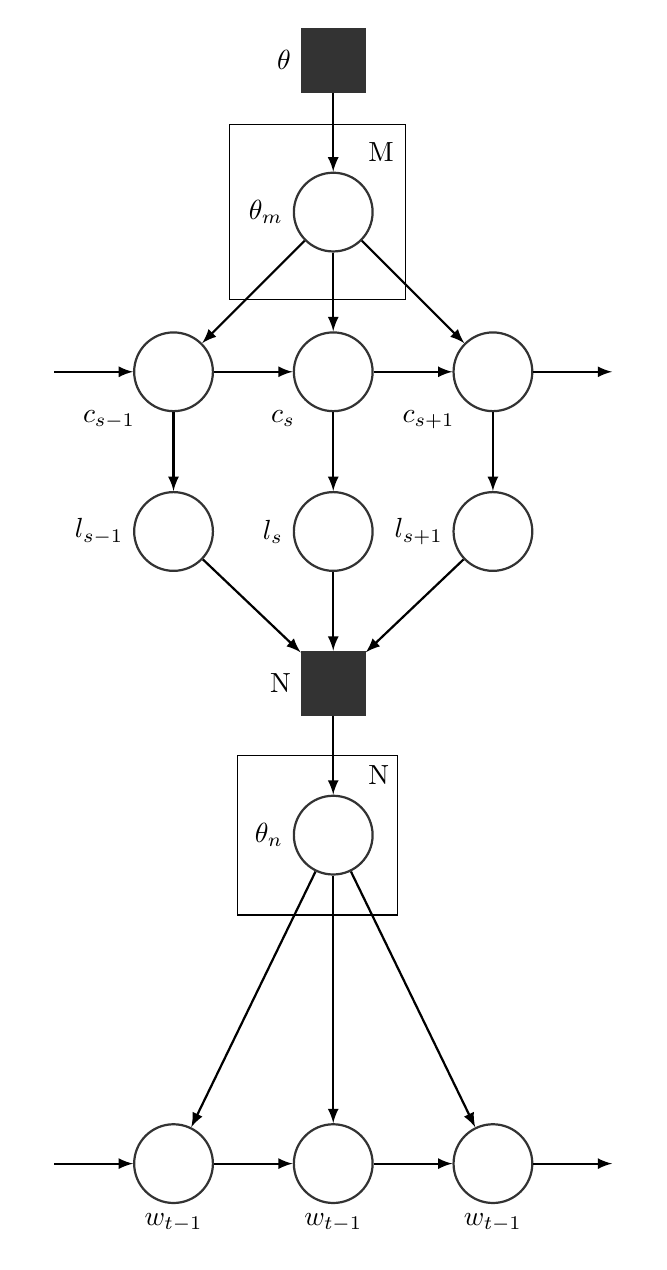
\begin{tikzpicture}
\tikzstyle{main}=[circle, minimum size = 10mm, thick, draw =black!80, node distance = 10mm]
\tikzstyle{square}=[rectangle, minimum size = 8mm, thick, draw=black!80, fill=black!80]
\tikzstyle{connect}=[-latex, thick]
\tikzstyle{box}=[rectangle, draw=black!100]
	\node[main] (c1) [label=below left:$c_{s-1}$] { };
	\node[circle] (c0) [left=of c1] { };
	\node[main] (c2) [right=of c1,label=below left:$c_{s}$] { };
	\node[main] (c3) [right=of c2,label=below left:$c_{s+1}$] { };
	\node[circle] (c4) [right=of c3] { };
	\node[main] (thetaM) [above=of c2,label=left:$\theta_{m}$] { };
	\node[square] (theta) [above=of thetaM,label=left:$\theta$] { };
	\path (theta) edge [connect] (thetaM); 
	\node[rectangle, inner sep=0mm, fit= (thetaM),label=above right:M,xshift=-2mm] {};
	\node[rectangle, inner sep=6mm,draw=black!100, fit= (thetaM),xshift=-2mm] {};
	\path (thetaM) edge [connect] (c1); 
	\path (thetaM) edge [connect] (c2); 
	\path (thetaM) edge [connect] (c3); 
	\path (c0) edge [connect] (c1); 
	\path (c1) edge [connect] (c2); 
	\path (c2) edge [connect] (c3); 
	\path (c3) edge [connect] (c4); 
	\node[main] (l1) [below=of c1,label=left:$l_{s-1}$] { };
	\node[main] (l2) [below=of c2,label=left:$l_{s}$] { };
	\node[main] (l3) [below=of c3,label=left:$l_{s+1}$] { };
	\path (c1) edge [connect] (l1); 
	\path (c2) edge [connect] (l2); 
	\path (c3) edge [connect] (l3); 
	\node[square] (n) [below=of l2,label=left:N] { }; 
	\path (l1) edge [connect] (n); 
	\path (l2) edge [connect] (n); 
	\path (l3) edge [connect] (n); 
	\node[main] (thetaN) [below=of n,label=left:$\theta_n$] { }; 
	\node[rectangle, inner sep=0mm, fit= (thetaN),label=above right:N,xshift=-2mm] {};
	\node[rectangle, inner sep=5mm,draw=black!100, fit= (thetaN),xshift=-2mm] {};
	\path (n) edge [connect] (thetaN); 
	\node[main] (w1) [below=7cm of l1,label=below:$w_{t-1}$] { };
	\node[circle] (w0) [left=of w1] { };
	\node[main] (w2) [below=7cm of l2,label=below:$w_{t-1}$] { };
	\node[main] (w3) [below=7cm of l3,label=below:$w_{t-1}$] { };
	\node[circle] (w4) [right=of w3] { };
	\path (w0) edge [connect] (w1); 
	\path (w1) edge [connect] (w2); 
	\path (w2) edge [connect] (w3); 
	\path (w3) edge [connect] (w4); 
	\path (thetaN) edge [connect] (w1); 
	\path (thetaN) edge [connect] (w2); 
	\path (thetaN) edge [connect] (w3); 
\end{tikzpicture}
\end{figure}

\end{document}
